\label{experiments}
\section{Experiments}

%In this section, we present the performance comparison of various backpressure variants on our simulator and provide a brief overview of the real-world implementation. All experiments are carried out on a 12 core Intel Xeon CPU E5-1650 machine with 32GB RAM operating at 3.20GHz. We tested a variety of networks with two main traffic matrices - all-to-all traffic matrix and random permutation traffic matrix. All presented results are for n-dimensional hypercubes with all-to-all traffic matrix. An n-dimensional hypercube consists of $2^{n}$ nodes, with each node connect to $n$ neighbors.
%
%\subsection{Basic backpressure algorithm}
%As a first step, we test the performance of basic backpressure protocol. In Figure~\ref{fig:basic}, we observe that the convergence time of the backpressure grows significantly with size. In hypercube-$7$ with $128$ nodes, the average convergence time is 18.5s. Hence this scheme is impractical for real-world implementation.
%\begin{figure}
%\centering
%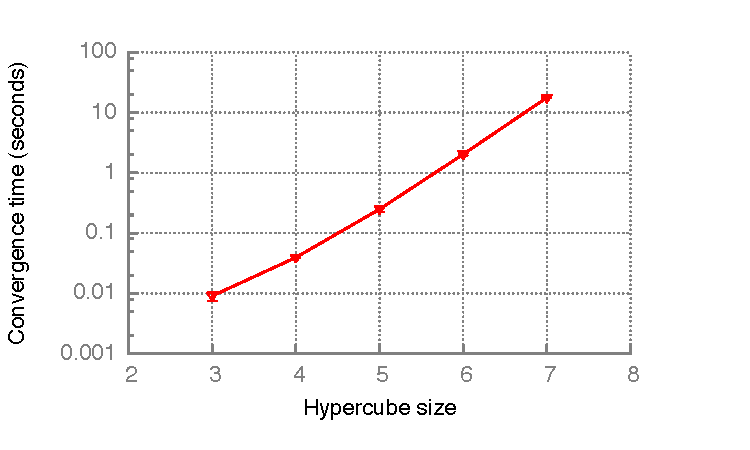
\includegraphics[width=3in, height=2in]{./figures/basic.pdf}
%\caption{\small Performance of basic backpressure algorithm}
%\label{fig:basic}
%\end{figure}
%
%\subsection{Variation with flow rate expansion}
%One of the proposed modifications in ~\cite{Srikant3} is expansion of input traffic by a constant traffic $\epsilon$. This expansion performed solely on the shadow queue traffic stresses the backpressure computation and forces it to reach equilibrium sooner, without impacting the actual traffic. As shown in Figure~\ref{fig:epsilon}, this improves the convergence time considerably. But, with an $\epsilon$ of 1.0, we can only test the system for a traffic load of $1/2$. In this case, for every real packet, $2$ packets are counted in the shadow queue. Thus we can operate only at half the capacity. In order to allow the network to function close to its capacity, we intend to use a heavy traffic matrix and $\epsilon = 0.1$  in the final implementation.
%
%\begin{figure}
%\centering
%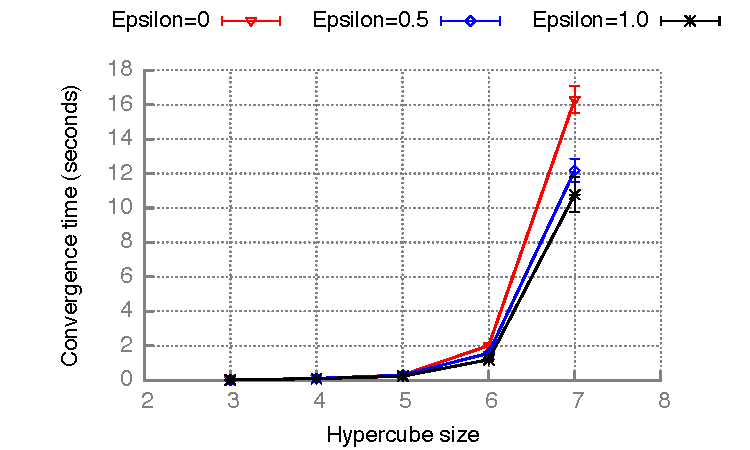
\includegraphics[width=3in, height=2in]{./figures/epsilon.pdf}
%\caption{\small Variation of convergence time with flow rate expansion}
%\label{fig:epsilon}
%\end{figure}
%
%
%\subsection{Variation with backpressure threshold}
%PARN~\cite{Srikant3} introduces a threshold for backpressure to force the flows to follow shorter path. In Figure~\ref{fig:M_1},we observe that introducing this factor has a significant impact on the performance. We observe that, while non-zero threshold can reduce the convergence time significantly, increasing M has diminishing returns. We also observed that very large M has a negative impact on the performance. Hence, we propose choosing $M=capacity$ as the optimal threshold, where capacity denotes the link capacity.
%
% 
%\begin{figure}
%\centering
%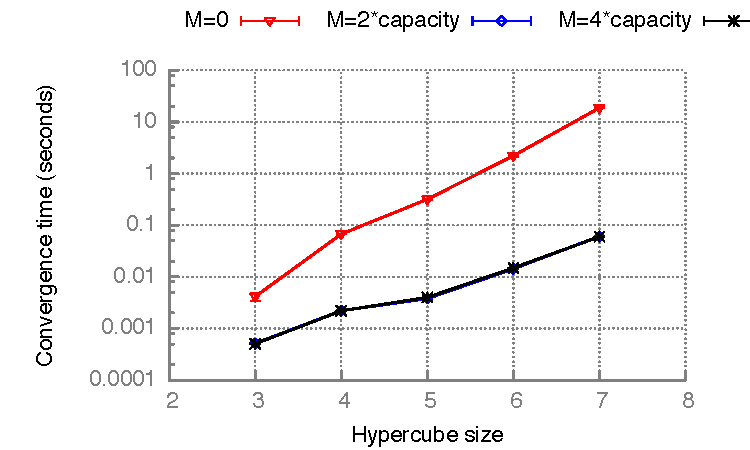
\includegraphics[width=3in, height=2in]{./figures/M_variation.pdf}
%\caption{\small Variation of convergence time with M}
%\label{fig:M_1}
%\end{figure}
%
%
%
%\subsection{Variation with Shadow Queue Initialization}
%The correctness of backpressure algorithm is independent of the initial value of shadow queues. Hence, we attempted to speed-up the convergence towards best paths by initializing the shadow queues with a multiple of path length. In Figure~\ref{fig:SQ}, we observe that initializing it with path length, improves the performance. But, if we initialize with a higher multiple of path-length it delays the convergence. This is expected since a large initial value creates a non-existent backpressure in the system and adversely affects the performance. On the other hand, initializing with path length helps the flows to follow the best path without exploring all other paths in the network. While the difference appears very small in an exponential scale on simulations, we expect that it can still be helpful in a real-world implementation.
%
%\begin{figure}
%\centering
%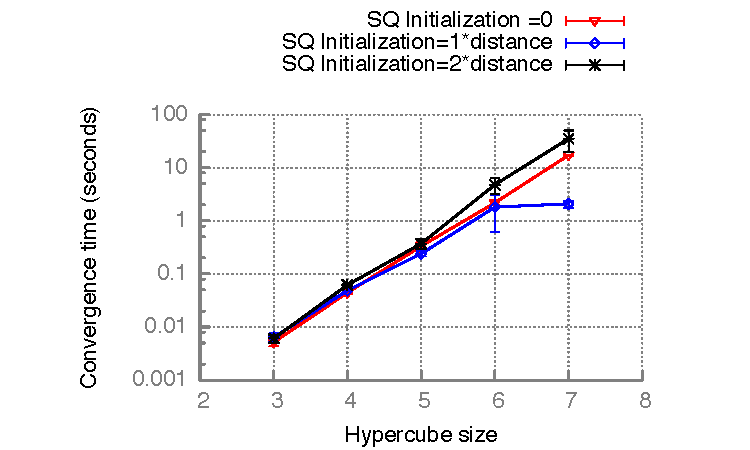
\includegraphics[width=3in, height=2in]{./figures/SQ.pdf}
%\caption{\small Variation of convergence time with Shadow Queue Initialization}
%\label{fig:SQ}
%\end{figure}
%
%\subsection{Variation with Proportional splitting}
%Finally, we compare proportional splitting and all the previously mentioned optimizations. In Figure~\ref{fig:prop}, we observe that replacing the best-destination transmission policy of the basic backpressure protocol with proportional splitting, improves its performance by an order of magnitude. These experiments were carried out with $M=0$ and $\epsilon=0.1$ to study the impact of proportional splitting with the proposed expansion in flow rate, ignoring the other significant player - backpressure threshold $M$.  
%\begin{figure}
%\centering
%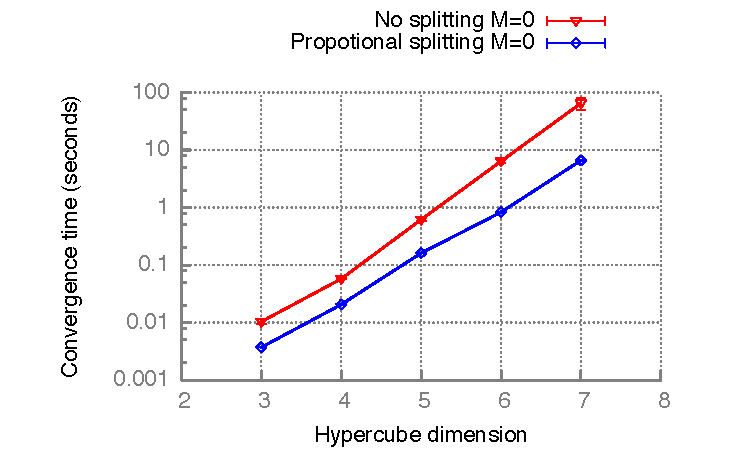
\includegraphics[width=3in, height=2in]{./figures/proportional.pdf}
%\caption{\small Variation of convergence time with Proportional splitting}
%\label{fig:prop}
%\end{figure}
%
%Finally, we add the significant contributors to the improvement of backpressure algorithm and compare the performance with the basic protocol. In Figure~\ref{fig:compare}, we observe that the optimized protocol performs three orders of magnitude better than the original version. 
%
%\begin{figure}
%\centering
%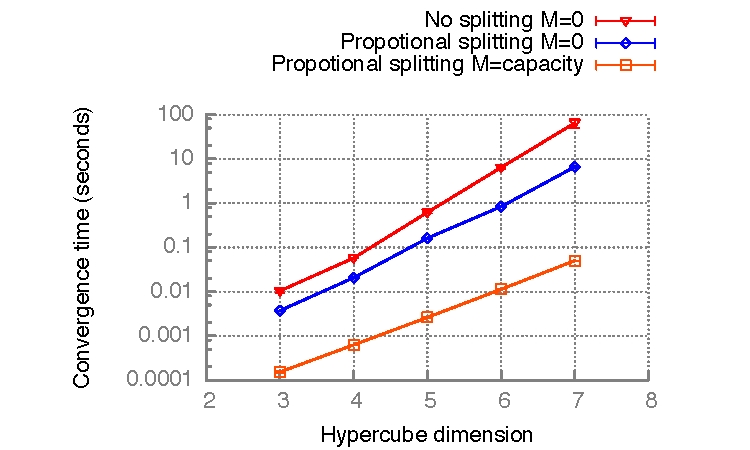
\includegraphics[width=3in, height=2in]{./figures/compare1.pdf}
%\caption{\small Comparison}
%\label{fig:compare}
%\end{figure}
%
%\subsection{Real implementation}
%%\begin{figure}
%%\centering
%%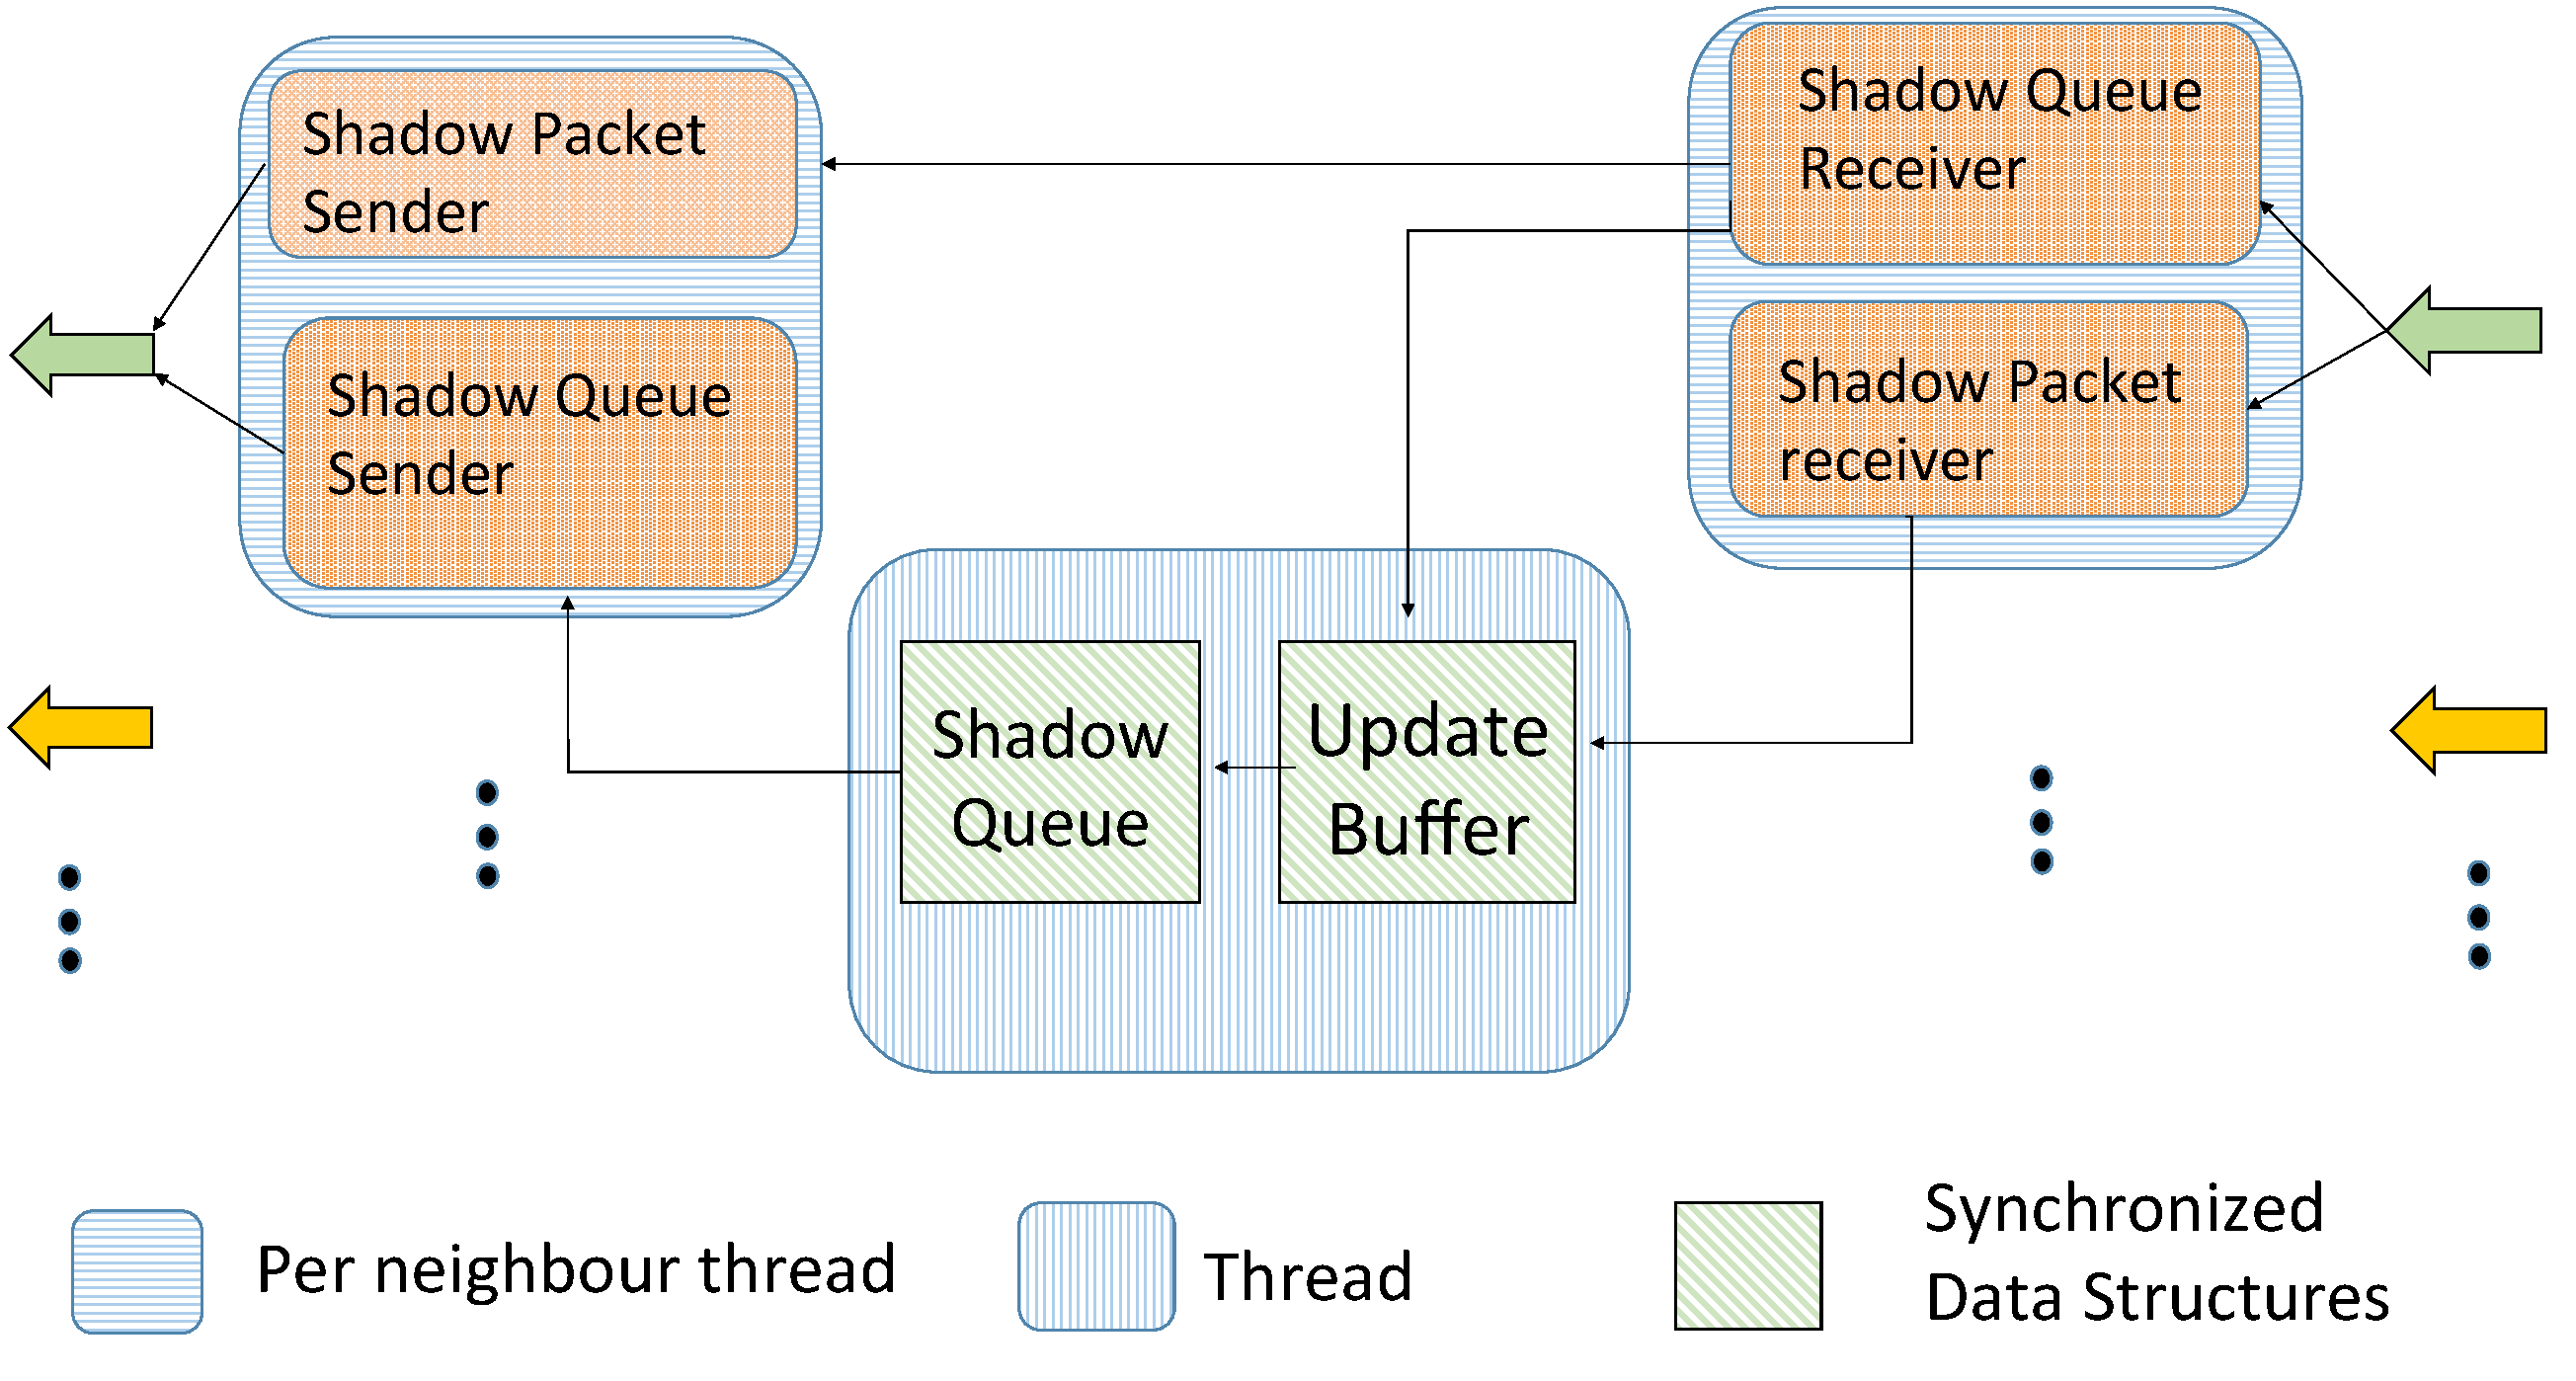
\includegraphics[width=3in, height=2in]{./figures/controlpath2.png}
%%\caption{\small Control path}
%%\label{fig:control}
%%\end{figure}
%%
%%\begin{figure}
%%\centering
%%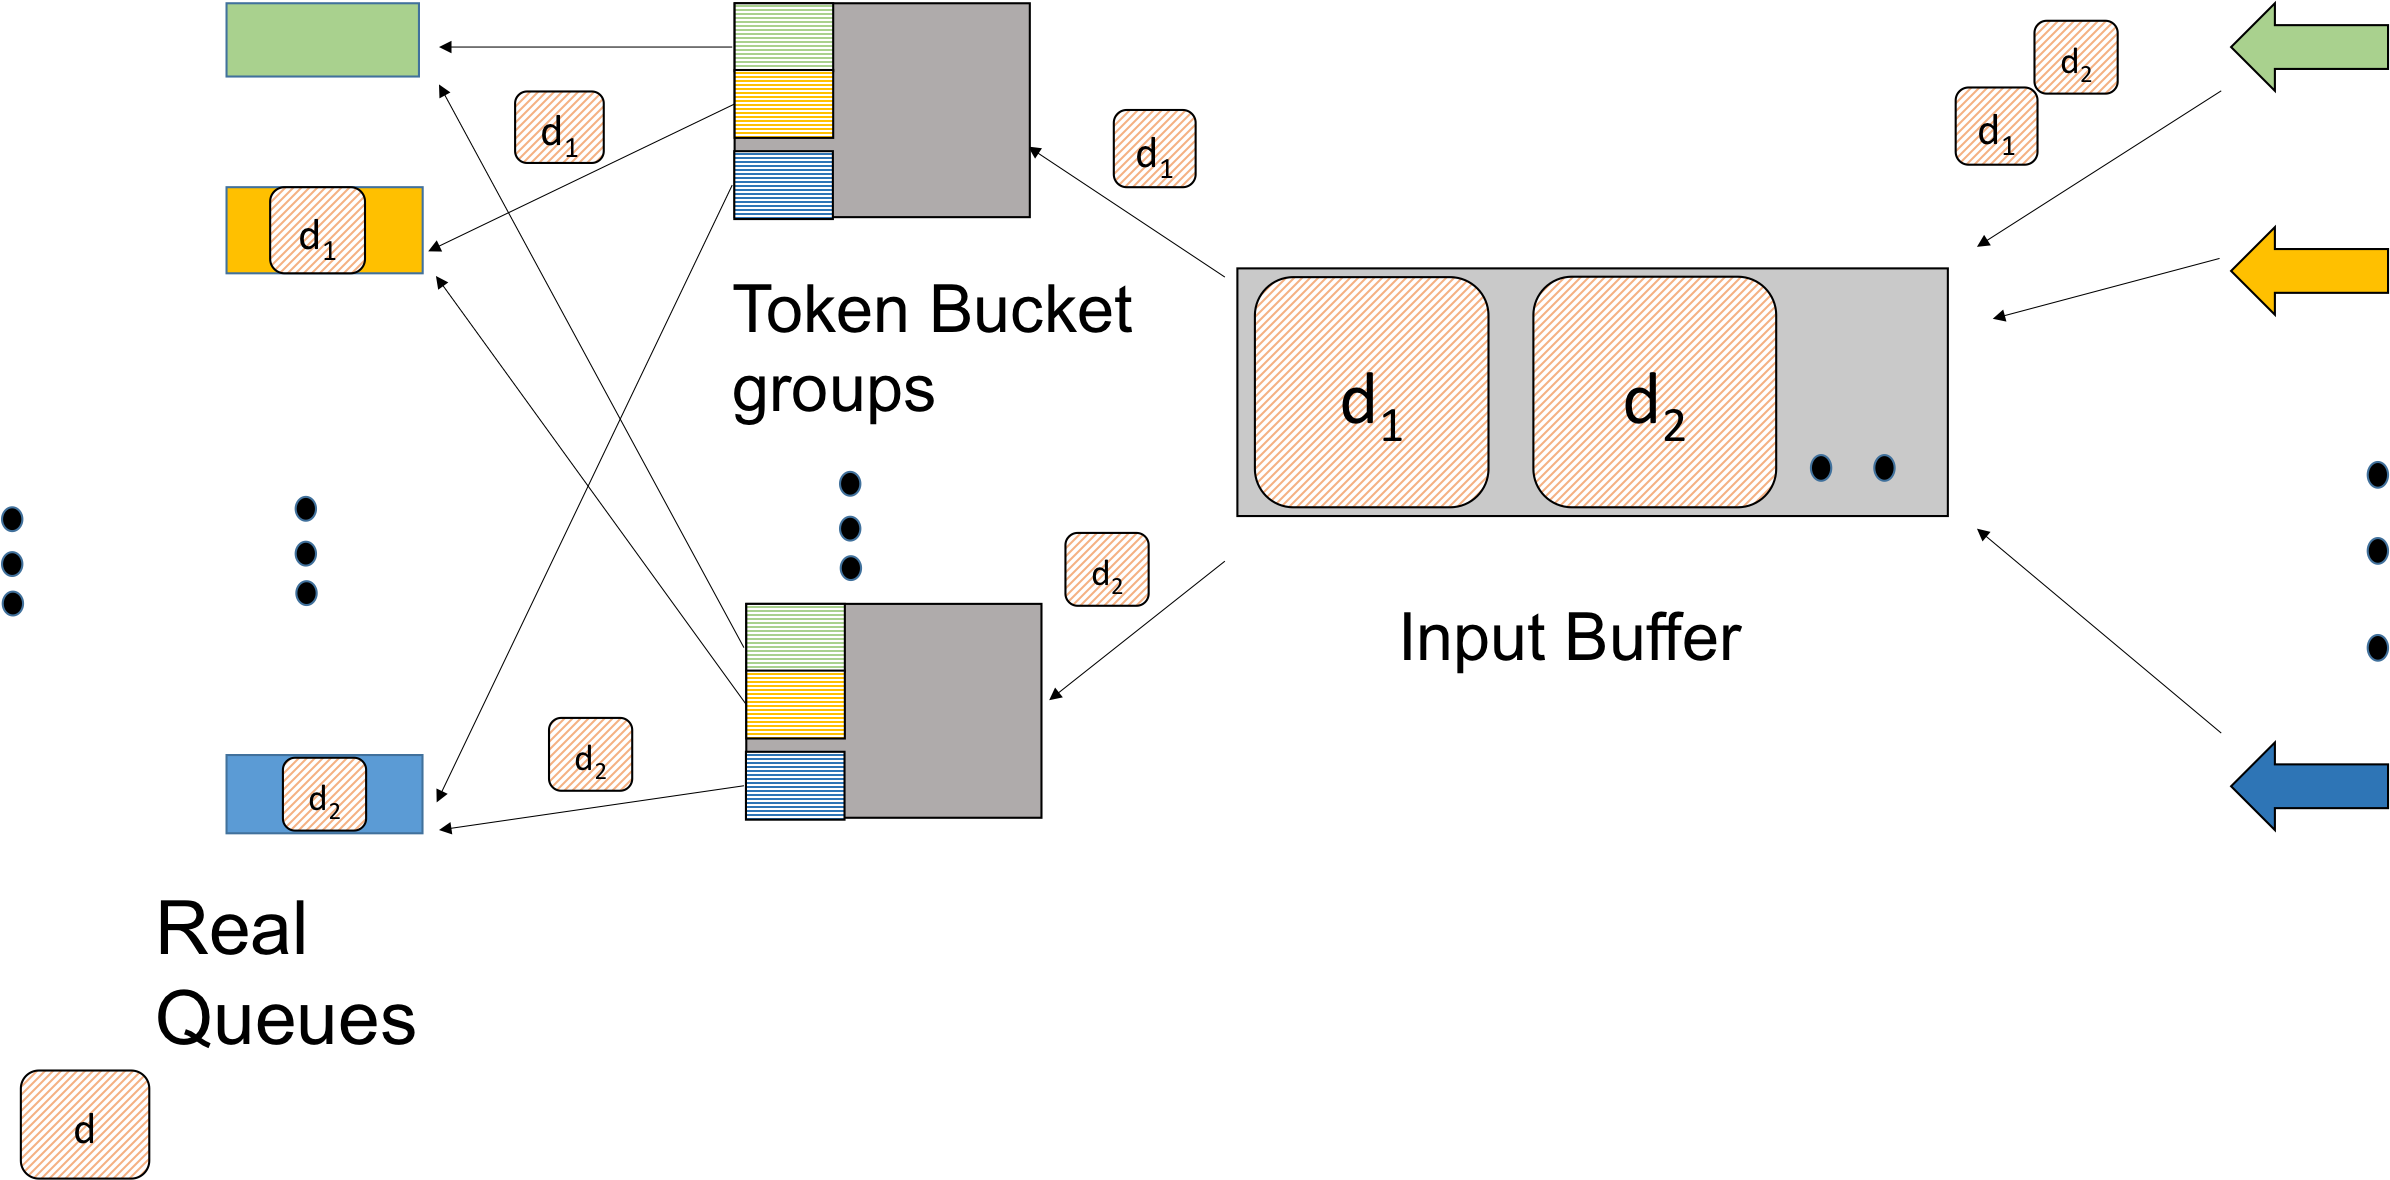
\includegraphics[width=3in, height=2in]{./figures/datapath3.png}
%%\caption{\small Data path}
%%\label{fig:data}
%%\end{figure}
%
\begin{figure*}
\centering
\begin{minipage}[b]{0.45\linewidth}
	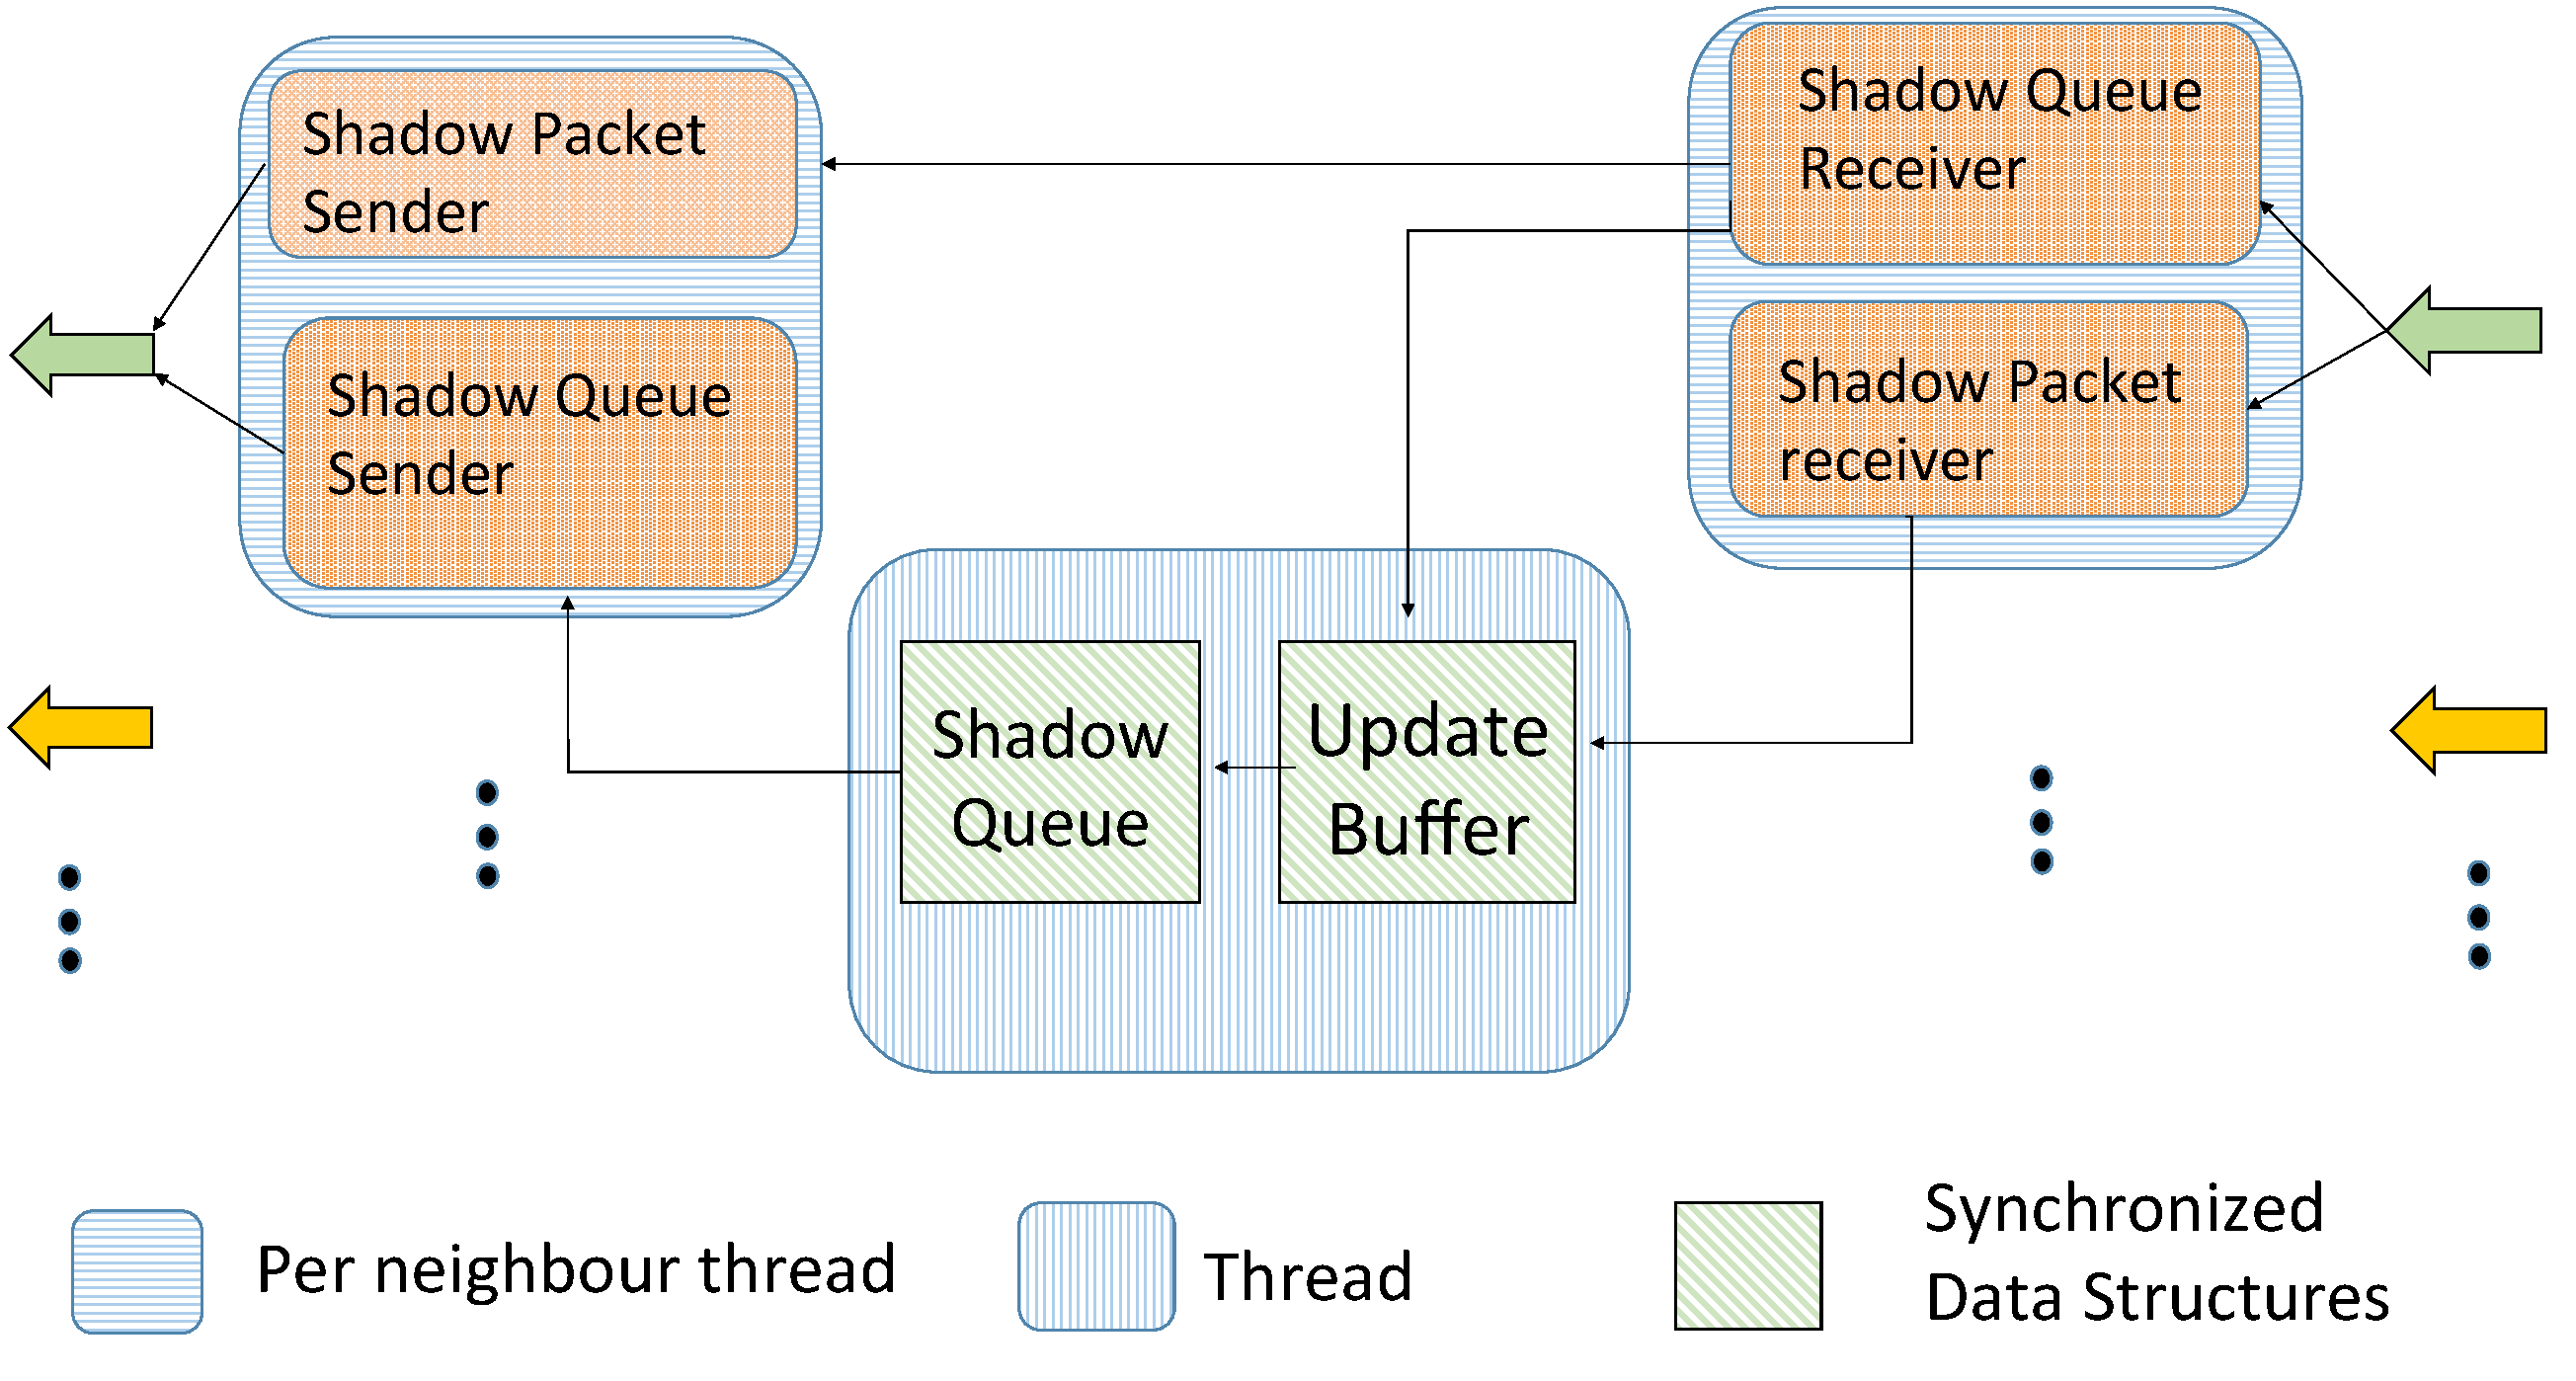
\includegraphics[width=2.4in]{./figures/controlpath2.pdf}
	\caption{Control path}
	\label{fig:control}
	\centering
	%\small Control path
\end{minipage}
\begin{minipage}[b]{0.45\linewidth}
	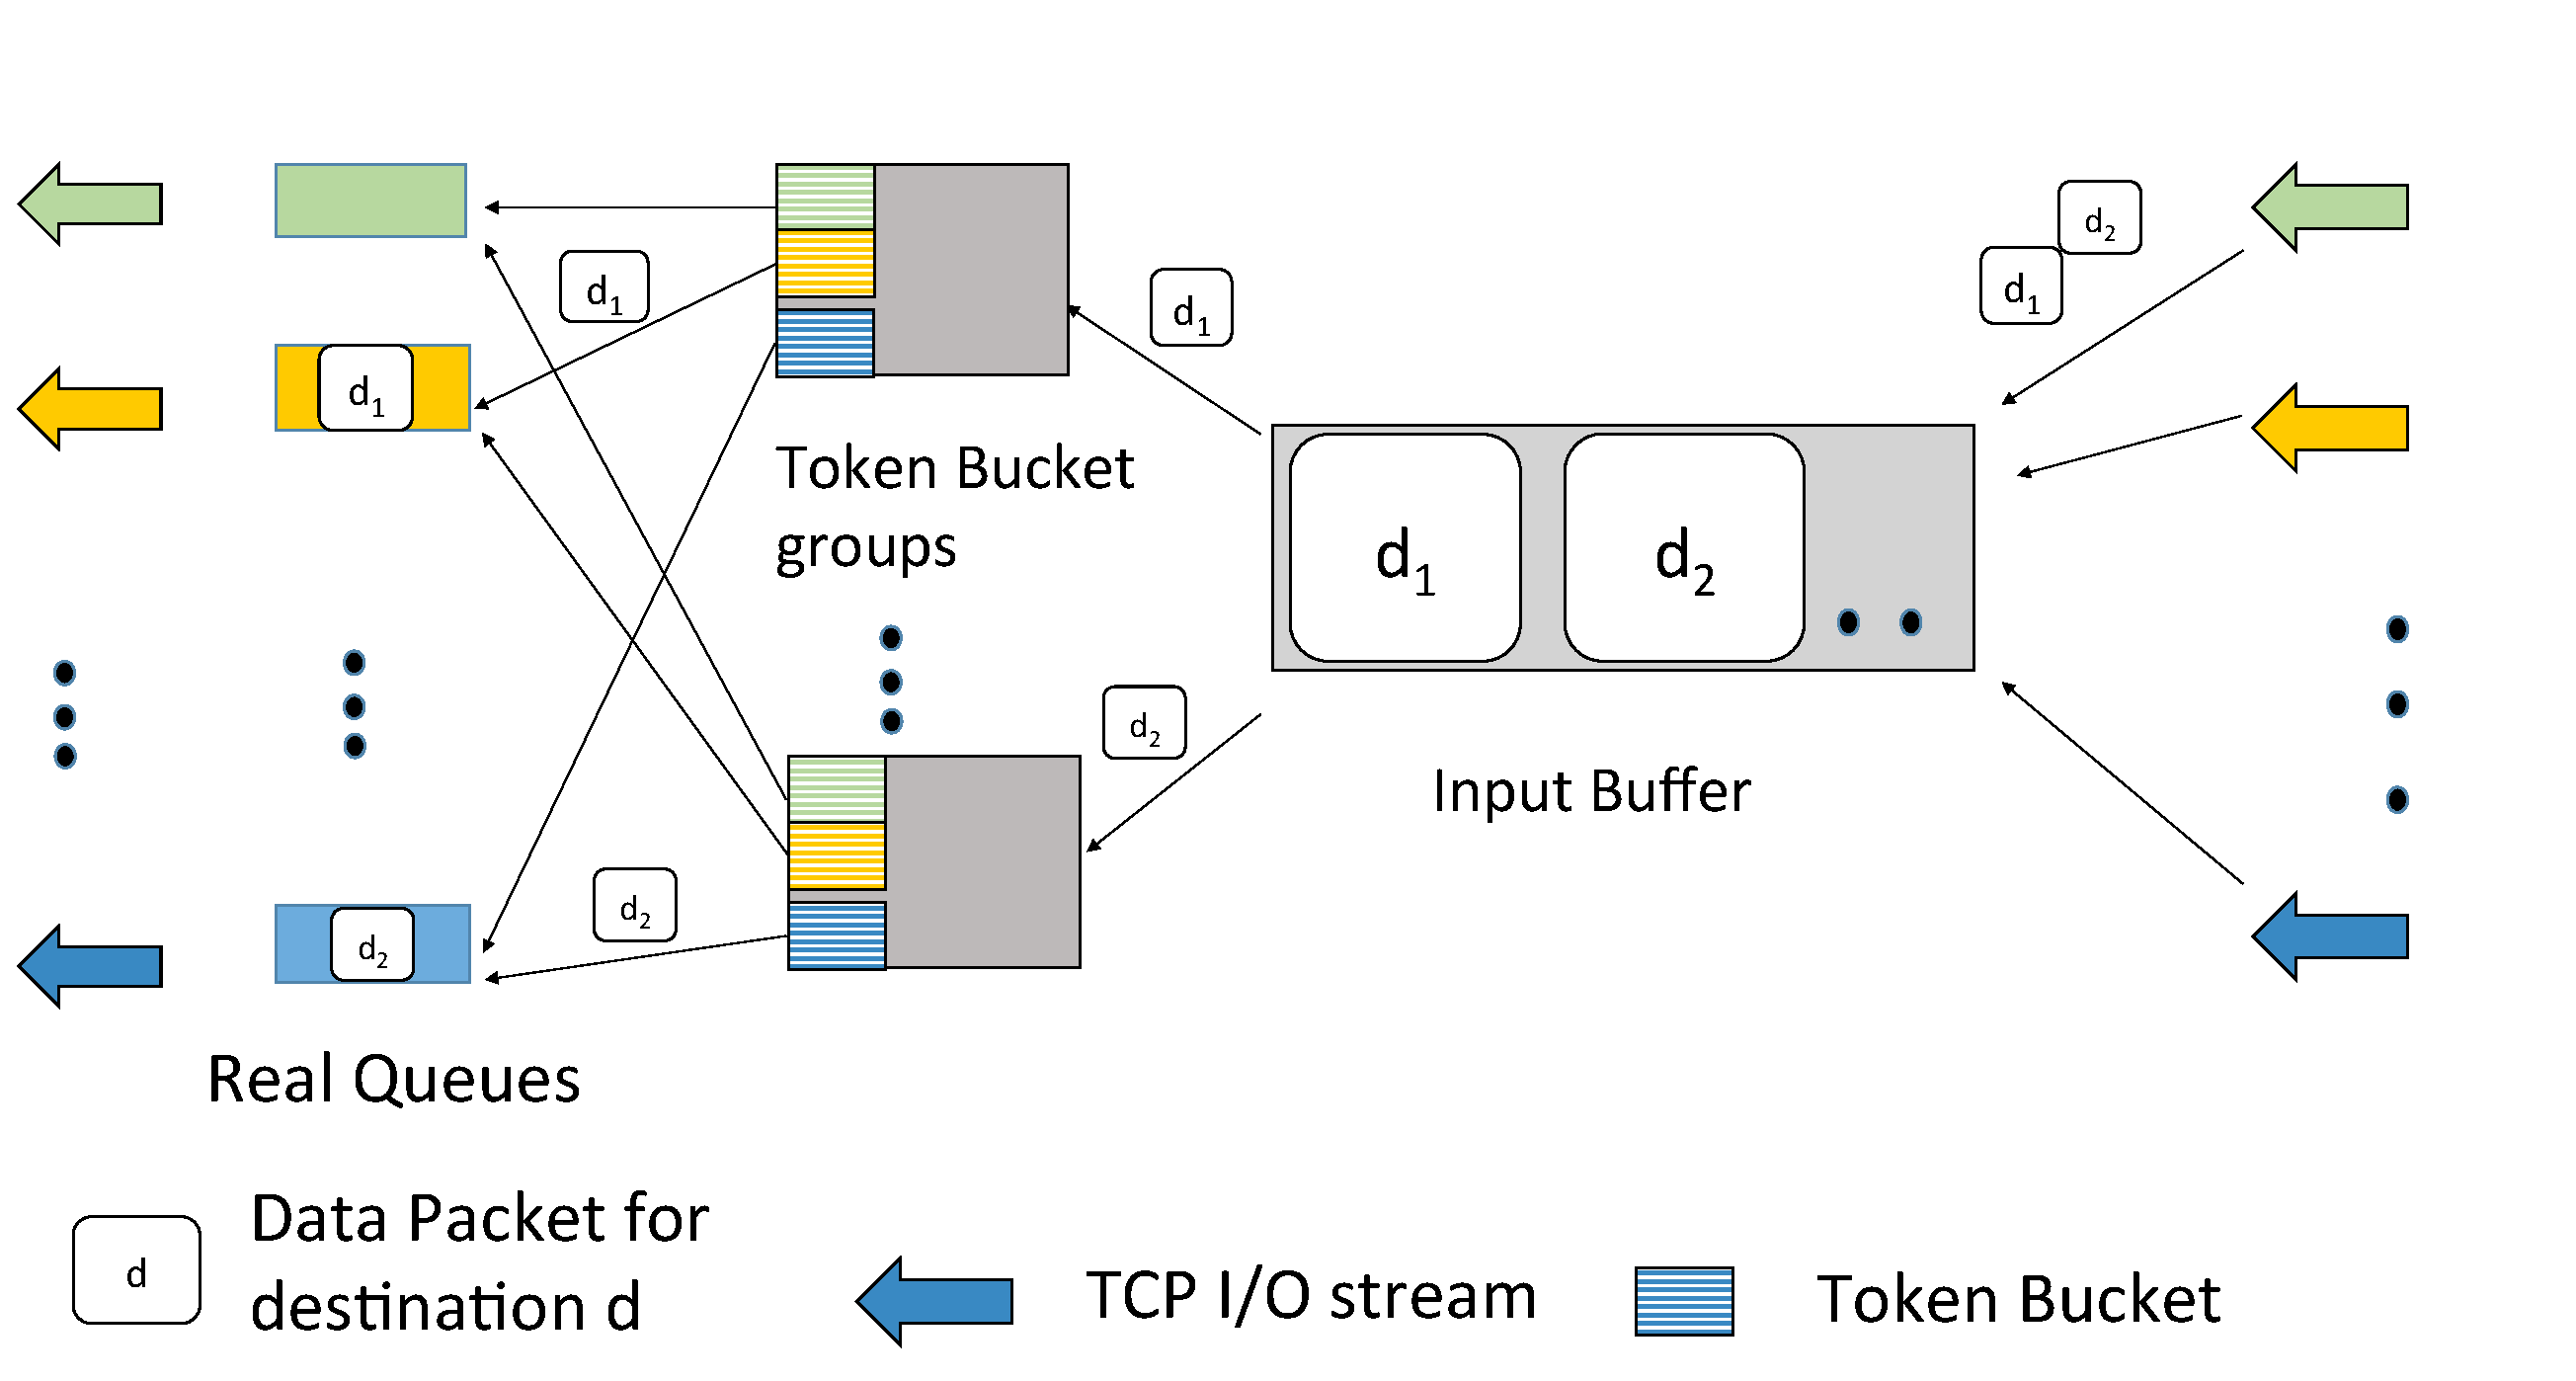
\includegraphics[width=2.4in]{./figures/datapath4.pdf}
	\caption{Data path}
	\label{fig:data} 
	\centering
	%\small Data path 
\end{minipage}
%\caption{\small Control path and data path in the real implementation}
%\label{fig:TCompare}
\end{figure*}


To observe the performance with realistic network conditions, we are implementing an overlay network over TCP/IP with nodes running variations of BackPressure routing protocol. We will test the system with different synchronization construct instead of assuming slotted time (complete synchronization). The rest of this section gives an overview of overlay node implementation. We will start by describing DataPath, followed by ControlPath.

DataPath(Figure~\ref{fig:data}) describes the routing and scheduling of Data packets, which is controlled by Control packets/path. Node keeps an incoming data channel per neighbor, each of which drains data packets into an \textit{input buffer} (FIFO queue) in a FIFO fashion. Packets from different channel may inter-mix in an arbitrary order depending on synchronization constructs for \textit{input buffer}. Like incoming channels, outgoing data channels are maintained for each neighbor, each of which drains packets from corresponding \textit{real queue} in FIFO fashion. A system wide thread transfers packets from \textit{input buffer} to an appropriate \textit{real queue} based on \textit{token buckets} ~\cite{Srikant3}. A \textit{token bucket group} is maintained for each destination, which contains \textit{token buckets} for each neighbor (or \textit{real queue}). A packet for destination \textit{d} goes to the smallest \textit{token bucket} in the corresponding group.

ControlPath (Figure~\ref{fig:control}) describes the flow of control information i.e. number of shadow packets transferred and shadow queue length advertisements. Like data channels, incoming and outgoing control channels are maintained for each neighbor. Control information, received from neighbors, is buffered before before it is applied to update nodes' own shadow queues. The way buffered updates are applied to shadow queues defines the synchronization construct. Waiting for updates from all the neighbors maps to slotted time assumption, which may result in high convergence time (since it is as slow as the slowest neighbor). The other extreme is to apply updates as soon as they are received, which is not proved to converge. We will test the system with different synchronization constructs. Note that updating shadow queue includes adjusting shadow queue lenghts, generating shadow packets (to be sent to neighbors) and updating token buckets, which determines the DataPath.
